\documentclass[main.tex]{subfiles}
\begin{document}

\subsection{Thorne's PSTF moment formalism}

The PSTF moment formalism was developed by \textcite{Thorne:1981feb} in order to give a way to consider the radiation energy transfer problem to an arbitrarily high degree of accuracy: it is fully relativistic, and --- in the presence of certain simmetries, such that it is possible to use its scalar-moments version, which will be developed in section \ref{par:scalar-moments} --- it gives rise to an infinite number of ordinary linear first-order differential equations for the various scalar moments, which can be truncated at a certain order.

We start by introducing the mathematical operations which will need to be applied to the moment tensors.

Given any tensor \(A^{\mu_1 \dots \mu_k} = A^{M_k}\) we can use the tensor \(h^{\mu\nu}\) to project it into the space-like subspace defined by the velocity \(u^\mu\):
\begin{equation}
    A^{M_k} \rightarrow \qty(A^{M_k})^P
    = \qty(\prod_{i=1}^k h^{\mu_i}_{\nu_i}) A^{M_k} \,.
\end{equation}

Then, we can take the symmetric part of any tensor as outlined in \Nameref{sec:notational-preface}:
\begin{equation}
    A^{M_k} \rightarrow \qty(A^{M_k})^S
    = A^{(M_k)} \,.
\end{equation}

We can select the trace-free part of a projected, symmetric tensor by
\begin{equation}
    A^{\mu_1 \dots \mu_k} \rightarrow \qty(A^{\mu_1 \dots \mu_k})^{TF}
    = \sum _{i=0}   ^{\lfloor k/2 \rfloor}
    (-1)^i \frac{k! (2k-2i-1)!!}{(k-2i)! (2k-1)!! (2i)!!}
    h^{(\alpha_1 \alpha_2} \dots h^{\alpha_{2i-1} \alpha_{2i}}
    A^{\alpha_{2i+1} \dots \alpha_k) \beta_1 \dots \beta_i}\,_{\beta_1 \dots \beta_i} \,.
\end{equation}

To see what this is doing, let us consider its action on a rank-two projected tensor: it is just the subtraction of its trace,
\begin{equation}
    A^{\mu\nu} \rightarrow A^{\mu\nu} - \frac{1}{3} h^{\mu\nu} A^{\rho}_\rho \,.
\end{equation}

Now, let us consider all the unit vectors \(n^\mu\) in the space normal to the velocity, which have \(n_\mu u^\mu = 0\) and \(n^\mu n_\mu = 1\). They span the sphere \(S^2\).

If we have a function \(F\colon S^2 \rightarrow \mathbb R\), we can decompose it into harmonics as:

\begin{equation}
    F(n) = \sum _{k=0}   ^{\infty}
    \mathscr F_{\alpha_1 \dots \alpha_k} \prod_{i=0}^k n^{\alpha_i}
\end{equation}
where the PSTF moments \(\mathscr F_{\alpha_1 \dots \alpha_k}\) can be computed as

\begin{equation} \label{eq:PSTF-moments-function-decomposition}
    \mathscr F_{\alpha_1 \dots \alpha_k} =
    \frac{(2k+1)!!}{4 \pi k!} \qty(\int F \prod_{i=0}^k n^{\alpha_i}  \dd{\Omega}  )^{TF} \,.
\end{equation}

In particular, the function we will apply this to is the distribution of EM radiation around the BH. So, we consider a photon, whose trajectory in spacetime is parameterized as \(\gamma(\xi)\), with a choice of \(\xi\) such that the photon's momentum is
\(
p = \dv*{}{\xi}
\).

Now, our observer has a timelike velocity \(u^\mu\). We can find a spacelike vector \(n^\mu\) corresponding to the space-like part of the movement of the photon, or

\begin{equation}
  p^\mu = (- u^\nu p_\nu) (u^\mu + n^\mu)\,.
\end{equation}

It must hold that \(u^\mu u_\mu = -1 \) while \(n^\mu n_\mu = +1 \) in order for \(p^\mu\) to be null-like.
Now, we define a parameter \(l\) which corresponds to the space distance the photon moved through in this frame (\(l\)  is \emph{not} covariant!)

\begin{equation}
    l = \int  (-u^\nu p_\nu) \dd{\xi}
\end{equation}
now, \(\dv*{}{l} \) is parallel to \(p\) but it has different length, in fact since \(\dv*{l}{\xi} = (-u^\nu p_\nu) \) it is \(\dv*{}{l} = (n^\mu + u^\mu) \partial_\mu\).

It holds (\cite[eq. 2.17]{Thorne:1981feb}, with the notation from \eqref{eq:covariant-acceleration-decomposition}), that

\begin{equation}
  \dv{\nu}{l}  = (u^\mu + n^\mu) \nabla_\mu (-p^\nu u_\nu) = - \nu \qty(n_\mu a^\mu  + \frac{\theta}{3} + n_\mu n_\nu \sigma^{\mu\nu})\,.
\end{equation}

We want to quantify the number density of photons in relation to their momentum. We assume the radiation in unpolarized, therefore for each unit \(h^3\) cell in phase space there can be 2 photons: so we denote the distribution function of the photons as \(2N (x^\mu, p^\mu)\).

It is known that the volume element \(\dd{V}_p = \dd[3]{p} / p^0 \) is Lorentz invariant (see \cite[box 22.5]{MisnerThorneWheeler:1973}).
We can write this using the photons' frequency \(\nu = - p^\mu u_\mu / h\) as \(\dd{V}_p = \nu \dd[]{\Omega} \dd{\nu} \).

Let us define the \emph{specific radiative intensity} as

\begin{equation}
  I_\nu = \frac{\delta E}{\delta A \delta  t \delta \nu \delta \Omega}
  = \frac{h \nu \delta N}{\delta A \delta  t \delta \nu \delta \Omega}
\end{equation}

where \(\delta A\) denotes an infinitesimal area the photons are coming through, \(\delta t\) an infinitesimal time, \(\delta \nu\) an infinitesimal photon frequency, \(\delta \Omega\) an infinitesimal solid angle.

Then, the number density of photons in phase space is \cite[figure 22.2]{MisnerThorneWheeler:1973}

\begin{equation}
  \frac{2N(x^\mu, p^\mu)}{h^3} = \frac{\delta N}{V_x V_p} =  \frac{\delta N}{h^3 \nu^2\delta A \delta  t \delta \nu \delta \Omega} = \frac{1}{h^4 \nu^3} I_\nu
\end{equation}

therefore \(I_\nu = 2 N \nu^3 h\).

Now, we want to describe the variation of the occupation number \(N\) with respect to the photons' trajectories' parameter \(l\). We encapsulate all possible effects into a source term \(\mathfrak S\):

\begin{equation}
    \mathfrak S \defeq \dv{}{l} 2N(x^\mu, p^\mu) =
    2 \qty(\pdv{N}{x^\mu} \dv{x^\mu}{l} + \pdv{N}{p^\mu} \dv{p^\mu}{l}  )
\end{equation}
since the occupation number can be thought of as just a function of the spatial components of the momentum.

Since \(\dv*{}{l} = (n^\mu + u^\mu) \partial_\mu\) and the covariant derivative of \(p^\gamma\) is zero, we can compute
\begin{equation}
  \dv{p^\gamma}{l} = (n^\mu + u^\mu ) \nabla_\mu p^\gamma - \Gamma ^\gamma _{\alpha \beta} p^\alpha (u^\beta + n^\beta)
  = - \Gamma ^\gamma _{\alpha \beta} p^\alpha (u^\beta + n^\beta)
\end{equation}
where the covariant derivative term vanishes since the photon's trajectory is a geodesic.

\paragraph{Moments' definitions}

In this subsection I will follow \textcite[]{Thorne:1981feb} in his usage of units where \(c=h=1\).

We define the (unprojected) \(k\)-th moments of radiative transfer:

\begin{subequations}
\begin{align}
   M _\nu ^{A_k}
   &\defeq \int 2N \frac{\delta (\nu - (-p^\nu u_\nu))}{\nu^{k-2}} \prod_i^k p^{\alpha_i} \dd{V_p} \\
   &= \int \qty(2N \nu^3) \frac{1}{\nu} \delta (\nu +p^\nu u_\nu) \prod_i^k \qty(\frac{p^{\alpha_i}}{\nu}) \qty(\nu \dd[]{\Omega} \dd[]{\nu})  \\
   &= \int  I_\nu \prod_i^k \qty(n^{\alpha_i} + u^{\alpha_i}) \dd[]{\Omega}\,. \label{eq:simplified-moment-definition}
\end{align}
\end{subequations}

In general, we can compute the \(k\)-th moments of any function just as here we computed those of \(2N = I_\nu / \nu^3\):
if we apply this procedure to the the source term \(\mathfrak S\) we get the following moments:

\begin{equation}
   S_\nu ^{A_k} = \nu^3 \int S \mathfrak S \prod_i^k (n^{\alpha_i} + u^{\alpha_i}) \dd[]{\Omega} \,.
\end{equation}

\paragraph{Redshift-adapted version}

\textcite[]{Thorne:1981feb} also defines a redshift-adapted version of the moments' definition: if \(R\) is a universal redshift functions, such that \(R (p^\nu u_\nu)\) is conserved along every photon geodesic \(p^\mu \nabla_\mu p^\nu = 0\), that is, \(R\) allows us to calculate the redshift between any two points \(A\), \(B\) which are connected by a geodesic as \(\nu_A / \nu_B = R_B / R_A\).

Then, we define \( M_f ^{A_k} =  M_{\nu} ^{A_k} / R\).

\paragraph{Frequency-integrated version}

We may not wish to consider the frequency dependence of the radiation, but instead to treat all radiative transfer ``in bulk'': to this end, we define the frequency-integrated moments:

\begin{equation}
   M ^{A_k} = \int M^{A_k} _\nu \dd{\nu}
\end{equation}
and the same is applied to the source moments \(S_\nu^{A_k} \rightarrow S^{A_k}\).

Since this includes the radiation intensity from all frequencies, we have direct interpretations for the first moments:

\begin{subequations}
\begin{align}
   M &= \int  I_\nu \dd{\Omega} \dd{\nu}   & \text{energy density of radiation}  \\
   M^\alpha &= \int I_\nu (n^\alpha + u^\alpha)\dd{\Omega} \dd{\nu}   & (M^0, M^i) = \text{(energy density of radiation, energy flux)}  \\
   M^{\alpha\beta} &= \int I (n^\alpha + u^\alpha)(n^\beta + u^\beta)\dd{\Omega} \dd{\nu}   & \text{stress-energy tensor of radiation.}
\end{align}
\end{subequations}

\paragraph{The moment equations}

These can be derived from the transport equation, see \cite[eq. 3.14]{Thorne:1981feb}. I present them only in the grey (frequency-integrated) case:

\begin{equation} \label{eq:grey-moment-equations}
  \nabla_\beta M^{A_k \beta} - (k-1) M^{A_k \beta \gamma} (\nabla_ \gamma u_\beta)= S^{A_k} \,.
\end{equation}

The moments (the frequency-integrated \(M^{A_k}\), but also the full moments \(M^{A_k}_\nu\) and the redshift-adapted ones \(M^{A_k}_f\)) satisfy the following:
\begin{subequations}
\begin{align}
  M^{A_k \beta}\,_\beta &= 0 \\
  u_\beta M^{A_k \beta} &= -M^{A_k} \\
  h_{\beta \gamma} M^{A_k \beta \gamma} &= M^{A_k} \,.
\end{align}
\end{subequations}

So, the \(k\)-th moment contains all the information about the \(l\)-th moments with \(l\leq k\); also, to get lower-order moments we take partial traces onto space- and time-like subspaces: therefore the unique information to the \(k\)-th moment, which is not redundantly expressed in lower-order moments, is in its PSTF part:

\begin{equation}
  \mathscr M ^{A_k} = \qty(M^{A_k}) ^{PSTF} \,.
\end{equation}

The same can be applied to \(M^{A_k}_\nu\) and \(M^{A_k}_f\), to the moment equations \eqref{eq:grey-moment-equations} and to the source moments \(S^{A_k} \rightarrow \mathscr S ^{A_k}\). Since we are taking the projection onto the space-like subspaces, we can simplify the expression of the PSTF moments: all the terms which contain at least a four-velocity vanish, therefore:

\begin{equation} \label{eq:trace-free-moments-definition}
  \mathscr M^{A_k} = \qty(\int I \prod_i n^{\alpha_i} \dd{\Omega})^{TF}
\end{equation}
where \(I = \int I_\nu \dd{\nu}\).
The first \emph{PSTF} moments also have physical interpretations:

\begin{subequations}
\begin{align}
   \mathscr M &= \int  I \dd{\Omega}    & \text{energy density of radiation}  \\
   \mathscr M^\alpha &= \int I n^\alpha\dd{\Omega}  & \text{energy flux of radiation}  \\
   \mathscr M^{\alpha\beta} &= \int I n^\alpha n^\beta \dd{\Omega}   & \text{shears in the stress-energy tensor of radiation.}
\end{align}
\end{subequations}

We can write the stress-energy tensor \(T^{\mu\nu} = M^{\mu\nu}\) with the PSTF moments (see \cite[eq. 4.9]{Thorne:1981feb}):

\begin{equation} \label{eq:PSTF-stress-energy-tensor-decomposition}
    T^{\mu\nu} = \mathscr M u^\mu u^\nu + 2 \mathscr M ^{(\mu} u^{\nu)}
    + \mathscr M ^{\mu\nu} + \frac{1}{3} \mathscr M h^{\mu\nu}
\end{equation}
and compare these to the expression of the components of the stress-energy tensor \eqref{eq:components-stress-energy-tensor} to get the following identifications:

\begin{subequations}
\begin{align}
  \mathscr M &= w = \rho  \label{eq:identification-PSTF-stress-energy-tensor-1}\\
  \mathscr M ^\mu &= w^\mu = -\kappa h^\mu _\sigma  \qty(\partial^\sigma T + T a^\sigma) \label{eq:identification-PSTF-stress-energy-tensor-2}\\
  \mathscr M^{\mu\nu} + \frac{1}{3} \mathscr M h^{\mu\nu}
  &= (p - \xi \theta)h^{\mu\nu} - 2 \eta \sigma^{\mu\nu} \label{eq:identification-PSTF-stress-energy-tensor-3}
\end{align}
\end{subequations}
and since the photons' paths are geodesics in this case \(\theta = 0\), for the components proportional to \(h^{\mu\nu}\) of equation \eqref{eq:identification-PSTF-stress-energy-tensor-3} we just get \(\rho = \frac[i]{1}{3} p\), which is what we expect for a photon gas.
For the traceless part of the equation, we get \(\mathscr M ^{\mu\nu} = -2 \eta \sigma^{\mu\nu}\).

\paragraph{The PSTF moment equations}

We want to express the grey moment equations \eqref{eq:grey-moment-equations} in terms of the PSTF moments. This can be done as follows: an expression can be found for the full moments in terms of the PSTF moments in \cite[eq. 4.10c]{Thorne:1981feb}:

\begin{equation}
  M^{A_k} = \sum_{l=0}^k \sum_{j=0}^{\lfloor \frac{k-l}{2} \rfloor}
  \frac{1}{(2j)!! (k-l-2j)!}  \frac{k!}{l!} \frac{(2l+1)!!}{(2l+1+2j)!!}
  \mathscr M^{(A_l} \prod_{i=l+1}^{l+2j-1} h^{\alpha_i \alpha_{i+1}}
  \prod_{x=l+2j+1}^k u^{\alpha_x)}
\end{equation}
where all the indices of the \(\mathscr M\), \(h\) and \(u\) are meant to be symmetrized.

We insert this into the moment equations and expand, making use of the decomposition of the covariant derivative of the 4-velocity \eqref{eq:covariant-acceleration-decomposition}.

Then, we should take the PSTF part of the equations. This yields a very complicated expression, so here I record only the implicit formula given in \textcite[eq. 4.11c]{Thorne:1981feb}:

\begin{equation} \label{eq:PSTF-grey-moment-equations}
  \begin{split}
    &\left( \nabla _\beta \mathscr M ^{A_k \beta} + u^\beta \nabla_\beta \mathscr M ^{A_k}
    + \frac{k}{2k+1} \nabla_{\alpha_k} \mathscr M ^{A_{k-1}}
    - (k-1) \mathscr M ^{A_k \beta \gamma} \sigma_{\beta \gamma} \right.
    - (k-1) \mathscr M ^{A_k \beta} a_\beta
    + \frac{4}{3} \mathscr M ^{A_k} \theta \\
    &+ \frac{5k}{2k+3} \mathscr M ^{A_{k-1} \beta} \sigma_\beta^{\alpha_k}
    - k \mathscr M ^{A_{k-1} \beta} \omega_\beta ^{\alpha_k}
    \left.+ \frac{k (k+3)}{2k+1} \mathscr M ^{A_{k-1}} a^{\alpha_k}
    + \frac{(k-1) k (k+2) }{(2k-1) (2k+1)} \mathscr M ^{A_{k-2}} \sigma^{\alpha_{k-1} \alpha_k} \right)^{PSTF} = \mathscr S ^{A_k} \,.
  \end{split}
\end{equation}

\paragraph{How to recover the intensity}

Once one has solved the PSTF grey moment equations, one can compute the intensity from the moments by comparing \eqref{eq:PSTF-moments-function-decomposition} and \eqref{eq:trace-free-moments-definition}:

\begin{equation}
  I = \sum _{k=0}   ^{\infty} \frac{(2k+1)!!}{4 \pi k!} \mathscr M^{A_k} \prod_{i=1}^k n_{\alpha_i}\,.
\end{equation}

\subsection{Generalized Bondi accretion}

\paragraph{Simplifications under assumptions of symmetry}

Instead of treating the general case as is done in \cite[]{Thorne:1981feb}, we describe the specific choices made under the assumption of spherical symmetry, following \textcite[]{ThorneFLammmangZytkow:1981feb}.

The fiducial frame defined in \eqref{eq:fiducial-frame} can still be used here: we  denote with a subscript ``fid'' the tensors expressed in that basis. We get the following expressions:

\begin{subequations} \label{eq:spherical-coordinates-simplifications}
\begin{align}
  a^\mu &= (0,\dv*{y}{r},0,0)_{\text{fid}} \\
  \theta &= - \frac{1}{r^2} \dv{}{r} \qty(r^2 v y)  \\
  \sigma_{\mu\nu} &= - \dv{}{r} \qty(\frac{vy}{r}) \frac{2r}{3} \begin{bmatrix}
  0   &   &   &  \\
     &  1 &   &  \\
     &   & -1/2  &  \\
     &   &   & -1/2
  \end{bmatrix} _{\text{fid}}
  = \sigma \begin{bmatrix}
  0   &   &   &  \\
     &  1 &   &  \\
     &   & -1/2  &  \\
     &   &   & -1/2
  \end{bmatrix} _{\text{fid}} \\
  \Gamma_{\theta r \theta} &= \Gamma_{\varphi r \varphi} = \frac{y}{r}\,.
\end{align}
\end{subequations}

We can see that the shear has been heavily simplified. This is a specific case of a general statement about the PSTF moments: in the spherically symmetric case, the \(k\)-th PSTF moment only has one independent component. This is because it satisfies the following identities:

\begin{subequations}
\begin{align}
  \mathscr M ^{A_k} &= 0 \text{ if } A_k \text{ contains an odd number of } \theta \text{s or } \varphi \text{s}  \label{eq:id1-pstf-spherically-symmetric}  \\
  \mathscr M ^{A_k \theta \theta} &= \mathscr M ^{A_k \varphi \varphi} = -\frac{1}{2} \mathscr M ^{A_k rr} \,. \label{eq:id2-pstf-spherically-symmetric}
\end{align}
\end{subequations}

Equation \eqref{eq:id1-pstf-spherically-symmetric} comes from the fact that an odd number of \(\theta\) or \(\varphi\) indices corresponds to and odd number of unit vectors which are integrated on the sphere (see the definition \eqref{eq:trace-free-moments-definition}): therefore the integrand is odd.

Equation \eqref{eq:id2-pstf-spherically-symmetric} comes from two observations:
first of all, the moments corresponding to indices \(\theta\) and \(\varphi\) respectively must be equal because of spherical symmetry; secondly the moments must be traceless, therefore the sum of the \(\theta \theta\), \(\varphi \varphi\) and \(rr\) moments must be zero (for any pair of indices).

So, with these every \(k\)-th moment is fully determined by the component \(\mathscr M ^{r\dots r}\) (\(k\) \(r\)s): therefore we give it a name: \(w_k\).
This fact is analogous to the statement that the only spherically symmetrical one of the spherical harmonics \(Y_{lm}\) is \(Y_{l0}\), therefore as in that case we have only one independent component for every \(l\).

\paragraph{Legendre polynomials complement}

The \(l\)-th Legendre polynomial is:

\begin{equation} \label{eq:legendre-polynomials}
    P_{l}(x)=\frac{1}{2^{l}} \sum_{k=0}^{\lfloor l / 2\rfloor} \frac{(-1)^{k}(2 l-2 k) !}{k !(l-k) !(l-2 k) !} x^{l-2 k} \,.
\end{equation}

We can see that the coefficient of \(x^l\) is \((2l)! / (2^l (l!)^2)\). We can rewrite this making use of the identities \((2n)! = (2n-1)!! (2n)!!\) and \((2n)!! = 2^n n!\),  as:

\begin{equation}
    \frac{(2l)!}{2^l (l!)^2} = \frac{1}{l!} \frac{(2l)!}{(2l)!!} = \frac{(2l-1)!!}{l!} = \frac{(2l+1)!!}{l! (2l+1)}
\end{equation}
which is equation \cite[eq. 5.7d]{Thorne:1981feb}.

In \textcite[eqs. 5.6]{Thorne:1981feb} we find the statement that:

\begin{equation} \label{eq:thorne-trace-free-integral-claim}
    \int_{-1}^1 I(\mu) P_k(\mu) \qty(\frac{(2k-1)!!}{l!})^{-1} \dd{\mu} = \qty(\int_{-1}^1  I(\mu) \prod_{i=1}^k n^r \dd{\mu})^{TF}
\end{equation}
where \(n^r\) denotes the radial component of a normal vector in spherical coordinates, \(P_k\) is the \(k\)-th Legendre polynomial and \(\mu = \cos \theta\) where \(\theta\) is the azimuthal coordinate of \(n\). \(I(\mu)\) is a generic function.

\paragraph{The scalar moments} \label{par:scalar-moments}

It can be shown, using the identity \eqref{eq:thorne-trace-free-integral-claim}  that the definition of \(w_k\) we gave is equivalent to

\begin{equation}
    w_k = \int_{-1}^1 I(\cos \theta) P_k(\cos \theta) \qty(\frac{(2k-1)!!}{l!})^{-1} 2 \pi\dd{\cos \theta}
\end{equation}
where \(P_k\) is the \(k\)-th Legendre polynomial \eqref{eq:legendre-polynomials}.
Then the first moments are:

\begin{subequations}
\begin{align}
  w_0 &= \int I \dd{\Omega} & \text{radiation energy density} \\
  w_1 &= \int I \cos \theta \dd{\Omega} & \text{radiation energy flux} \\
  w_2 &= \int I \qty(\cos^2 \theta - \frac{1}{3}) \dd{\Omega} & \text{radiation shear stress.}
\end{align}
\end{subequations}

We can explicitly write the radiation stress-energy tensor in terms of the \(w_k\) using \eqref{eq:PSTF-stress-energy-tensor-decomposition}:

\begin{equation} \label{eq:radiation-stress-energy-tensor-fiducial}
    T^{\mu\nu}_{\text{radiation}} = \begin{bmatrix}
    w_0   & w_1  & 0  & 0 \\
    w_1   & \frac{1}{3}w_0 + w_2  &  0  & 0 \\
      0 & 0  &  \frac{1}{3}w_0 -\frac{1}{2}w_2 &  \\
      0 & 0  &   & \frac{1}{3}w_0 -\frac{1}{2}w_2
  \end{bmatrix} _{\text{fid}}\,.
\end{equation}

\paragraph{The source moments}

We can get an explicit formula for the source moments \(s_k = \mathscr S ^{r\dots r}\) (\(k\) \(r\)s) with the same procedure which was used in paragraph \nameref{par:scalar-moments}:
we get

\begin{equation}
    s_k = \int_{-1}^1 \dv{I}{l} (\cos \theta) P_k(\cos \theta) \qty(\frac{(2k-1)!!}{l!})^{-1} 2 \pi\dd{\cos \theta}
\end{equation}
where \(\dv*{I}{l} = \int \mathfrak S \nu^3 \dd{\nu}\) is the frequency-integrated  source term in the transfer equation.

% \begin{greenbox}
%   The derivative \(\dv*{I}{l}\) first appears in \cite[]{Thorne:1981feb} without any indices, then in \cite[section 6]{Thorne:1981feb} it gets the index ``source'', while in \cite[eq. 15]{ThorneFLammmangZytkow:1981feb} it appears with an index ``interaction'' (and the derivative becomes a proper time one).
%
%   It is not clear to me whether these all represent the same thing, or what the indices are trying to say.
% \end{greenbox}

\paragraph{The simplified moment equations}

It is possible to write equations \eqref{eq:PSTF-grey-moment-equations} explicitly in terms of the \(w_k\) and of derivatives wrt the fiducial basis: one gets \cite[eq. 5.10c]{Thorne:1981feb}

\begin{equation} \label{eq:scalar-PSTF-moment-equations}
  \begin{split}
    \pdv{w_{k+1}}{\hat{r}} &+[(2-k) a+(k+2) b] w_{k+1}+\pdv{w_k}{\hat{t}}+\left[\frac{4}{3} \theta+\frac{5 k(k+1)}{2(2 k-1)(2 k+3)} \sigma\right] w_{k} + \\
    &+\frac{k^{2}}{(2 k-1)(2 k+1)} \pdv{w_{k-1}}{\hat{r}}+\frac{k^{2}[(k+3) a+(1-k) b]}{(2 k-1)(2 k+1)} w_{k-1} +  \\
    &-\frac{3}{2}(k-1) \sigma w_{k+2}+\frac{3(k-1)^{2} k^{2}(k+2)}{2(2 k-3)(2 k-1)^{2}(2 k+1)} \sigma w_{k-2} = s_k
    \end{split}
\end{equation}
where \(a = \dv*{y}{r} = \sqrt{a^\mu a_\mu}\) is the magnitude of the 4-acceleration, \(b = y/r\) is the extrinsic curvature, \(\theta\) is the expansion velocity, \(\sigma\) is the scalar shear --- the largest eigenvalue of the shear matrix. Explicit expressions for these are found in  \eqref{eq:spherical-coordinates-simplifications}.

\textcite[]{NobiliTurollaZampieri:1991dec} only used the first two of the moment equations, so here is how the expression is simplified for \(k=0,1\):
for \(k=0\) we get:

\begin{equation}
    \pdv{w_{1}}{\hat{r}} +2( a+ b) w_{1}+\pdv{w_0}{\hat{t}}+\frac{4}{3} \theta w_{0} + \frac{3}{2} \sigma w_{2} = s_0\,.
\end{equation}

For \(k=1\) we get:

\begin{equation}
    \pdv{w_{2}}{\hat{r}} + (a+3 b) w_{2}+\pdv{w_1}{\hat{t}}+\left[\frac{4}{3} \theta+ \sigma\right] w_{1} +\frac{1}{3} \pdv{w_{0}}{\hat{r}}+\frac{4 a}{3} w_{0} = s_1\,.
\end{equation}

These have to be simplified further to be used: specifically, they can be expressed with respect to \(r\), \(v\), \(y\).

\paragraph{Simplifying the moment equations further}

% Following \textcite[]{ThorneFLammmangZytkow:1981feb}.

Because of the hypothesis of stationarity, we can express the derivatives in \eqref{eq:scalar-PSTF-moment-equations} as:

\begin{subequations}
\begin{align}
  \pdv{}{\hat{t}} &= \frac{\gamma^2}{y} \pdv{}{t} - yv \pdv{}{r} = - yv \pdv{}{r}  \\
  \pdv{}{\hat{r}} &= -v \frac{\gamma^2}{y} \pdv{}{t} + y \pdv{}{r} = y \pdv{}{r}\,.
\end{align}
\end{subequations}

Now, we can make the scalar PSTF moment equations \eqref{eq:scalar-PSTF-moment-equations} fully explicit: denoting derivation with respect to \(r\) with a prime, we have
\begin{subequations}
\begin{align}
  y \dv{w_1}{r} + 2 \qty(\dv{y}{r} + \frac{y}{r}) w_1
  -yv \dv{w_0}{r}
  - \frac{4}{3} \frac{w_0}{r^2} \dv{}{r}\qty(r^2 v y)
  - w_2 r \dv{}{r}\qty(\frac{vy}{r}) &= s_0  \\
  y \dv{w_2}{r} + \qty(\dv{y}{r} + \frac{3y}{r})w_2
  - yv \dv{w_1 }{r} - \frac{4}{3r^2} \dv{}{r}\qty(r^2 vy) w_1
  - \frac{2r}{3} \dv{}{r}\qty(\frac{vy}{r}) w_1
  + \frac{y}{3} \dv{w_0}{r} + \frac{4}{3} \dv{y}{r} w_0
  &= s_1\,.
\end{align}
\end{subequations}

We can simplify these by expanding the derivatives of products \(\dv{(vyr^2)}{r}\) and \(\dv{(vy/r)}{r}\):
\begin{subequations} \label{eq:NTZ91-moment-equations-spherical}
\begin{align}
  y \dv{w_1}{r} + 2 \qty(\dv{y}{r} + \frac{y}{r}) w_1
  -yv \dv{w_0}{r}
  - \frac{4}{3} w_0 \qty(\dv{(v y)}{r} + \frac{2vy}{r})
  - w_2 \qty(\dv{(vy)}{r} - \frac{vy}{r}) &= s_0  \\
  y \dv{w_2}{r} + \qty(\dv{y}{r} + \frac{3y}{r})w_2
  - yv \dv{w_1 }{r}
  - 2 w_1 \qty(\dv{(vy)}{r} + \frac{vy}{r})
  + \frac{y}{3} \dv{w_0}{r} + \frac{4}{3} \dv{y}{r} w_0
  &= s_1\,.
\end{align}
\end{subequations}

Equations \eqref{eq:NTZ91-moment-equations-spherical} are the ones which appear in  \textcite[eq. 4]{NobiliTurollaZampieri:1991dec} and which are reported in equation \eqref{eq:NTZ91-moment-equations-logarithmic}, with the notation of primes denoting differentiation with respect to \(\log r\):\footnote{Do note that in the paper \cite[]{NobiliTurollaZampieri:1991dec} the letter \(r\) is used to denote the adimensional radial coordinate \(r / (2M)\).}

\begin{subequations} \label{eq:NTZ91-moment-equations-logarithmic}
    \begin{align}
        w_{1}^{\prime}-v w_{0}^{\prime}
        -v w_{2}\left[\frac{(v y)^{\prime}}{v y}-1\right]
        +2 w_{1}\left(1+\frac{y^{\prime}}{y}\right)
        -\frac{4}{3} v w_{0}\left[\frac{(v y)^{\prime}}{v y}+2\right]&=\frac{r s_{0}}{y} \\
        w_{2}^{\prime}-v w_{1}^{\prime}+\frac{1}{3} w_{0}^{\prime} +w_{2}\left(3+\frac{y^{\prime}}{y}\right)-2 v w_{1}\left[\frac{(v y)^{\prime}}{v y}+1\right]+\frac{4}{3} \frac{y^{\prime}}{y} w_{0} &=\frac{r s_{1}}{y}\,.
    \end{align}
\end{subequations}

\paragraph{Some properties of the accretion variables}

From equation \eqref{eq:mass-conservation-integral} we can find an expression \cite[eq. 18a]{ThorneFLammmangZytkow:1981feb} for \(y\) which only depends on \(r\) and constants:

\begin{equation}
  y = \sqrt{y^2 \qty(1 - v^2 + v^2)}
  = \sqrt{\qty(\frac{y^2}{\gamma^2}) + y^2 v^2}
  = \sqrt{\qty(1 - \frac{2M}{r}) + \qty(\frac{\dot{M}}{4 \pi r^2 \rho_0})^2}
\end{equation}
therefore by the continuity equation \(v\) can also be expressed in terms of \(r\) and constants:

\begin{equation}
  v = \frac{\dot M}{4 \pi r^2 \rho_0 y(r)}\,.
\end{equation}

\paragraph{The source term}

The source term can be written \cite[eq. 15]{ThorneFLammmangZytkow:1981feb} as

\begin{equation} \label{eq:source-term}
  s_k = \frac{l! (2l+1)}{(2l+1)!!} \int_{-1}^1 \dv{I}{l} P_k(\mu) 2 \pi \dd{\mu}\,.
\end{equation}

% \begin{greenbox}
%   Why is this a proper-time derivative of the intensity instead of a derivative wrt to the photon spatial distance parameter \(l\) as in \cite[]{Thorne:1981feb}?
% \end{greenbox}

The general relation for the change in intensity is

\begin{equation}
  \dv{I_\nu}{l} = \rho_0 \qty(\varepsilon_\nu - \kappa_\nu I_\nu )
\end{equation}
where \(\rho_0\) is the rest mass density, while \(\varepsilon_\nu\) and \(\kappa_\nu\) are the specific coefficients of emission and absorption. If we integrate this relation over all frequencies and take its \(k\)-th moment, we get

\begin{equation} \label{eq:opacity-emissivity-definition}
  s_k = \rho_0 (\varepsilon_k - \kappa_k w_k)
\end{equation}
where \(w_k\) are the PSTF scalar moments, \(\varepsilon_k\) is the \(k\)-th moment of emissivity and \(\kappa_k\) is the \(k\)-th moment of opacity of the gas.

Equation \eqref{eq:opacity-emissivity-definition} can be taken to be a practical definition of \(\varepsilon_k\) and \(\kappa_k\); we do the integral in \eqref{eq:source-term} and get constant terms and terms proportional to \(w_k\), which we split into the two terms on the RHS of \eqref{eq:opacity-emissivity-definition}.

We will only consider the \(k=0\) and \(k=1\) moments.
If the emission is isotropic, then the emissivity moment \(\varepsilon_1\) is 0 since its definition contains an integral of the product of an even and odd function.

Because of this, we just call the one moment we need \(\varepsilon = \varepsilon_0\).

The source moments given in \cite[eq. 6]{NobiliTurollaZampieri:1991dec} are:

\begin{subequations}
\begin{align}
  s_0 &= \rho_0 \qty(\varepsilon - w_0 \qty(\kappa_0 - \kappa_{\text{es}} \frac{4 k_B}{m_e} (T - T_\gamma)))  \\
  s_1 &= - \rho_0 w_1 \kappa_1
\end{align}
\end{subequations}
with

\begin{equation}
    T_\gamma = \frac{1}{4 k_B} \frac{\displaystyle \int_0^\infty h \nu w_0 (r, \nu) \dd{\nu}}{\displaystyle \int_0^\infty w_0 (r, \nu) \dd{\nu}}\,.
\end{equation}

Do note that the determination of the radiation temperature \(T_\gamma\) with the definition given is impossible if only the frequency-integrated transfer problem is solved: a reasonable approximation has to be made in order to compute it in this case.

\textcite[eq. 17]{NobiliTurollaZampieri:1991dec}, following the works of Park and Ostriker, propose the following differential equation for the determination of the logarithmic derivative of \(T_\gamma\) when the temperature profile is known:
%
\begin{equation} \label{eq:T-gamma-differential-equation}
  \frac{T_\gamma ^{\prime}}{T_\gamma} = \frac{4 k_B T \max (\tau, \tau^2)}{m_e} \frac{T - T_\gamma}{T}\,.
\end{equation}
%
where \(\tau\) is the adimensional optical depth. This differential equation has to be solved simultaneously with the ones which will be found later.

Furthermore, we use the facts that \(\varepsilon / \kappa_0 = a T^4\) if there is thermodynamic equilibrium and that we have the following expression for the emissivity \(\varepsilon\) in terms of the cooling function \(\Lambda (T)\) (given in \eqref{eq:cooling-function-NTZ91}):

\begin{equation}
    \varepsilon = \frac{\rho_0 \Lambda (T)}{m_p^2}
\end{equation}
to write the source term \(s_0\) as

\begin{equation}
    s_0 = \frac{\rho_0^2 \Lambda (T)}{m_p^2} \qty(1 - \frac{w_0}{aT^4}) + \rho_0 \kappa_{\text{es}} w_0 \frac{4 k_B}{m_e} (T - T_\gamma)\,.
\end{equation}

As for the \(s_1\) term, we model \(\kappa_1\) as

\begin{equation}
  \kappa_1 = \kappa_{\text{es}} + \expval{\kappa_{\text{ff}}}
  = \kappa_{\text{es}} + \SI{6.4e22}{\centi\metre\square\per\gram} \rho_0 T^{-7/2}
\end{equation}

where the second term is the conventional approximation of the \emph{Rosseland mean opacity} computed taking into account only free-free transitions: the definition of the RMO is a harmonic mean of the opacities at every frequency, weighted by the derivatives with respect to temperature of the Planck function\footnote{The Planck function \cite[eq. 1.51]{RybickiLightman:2004}, here given reintroducing \(c\) explicitly,
\[
B_\nu = \frac{2h \nu^3 c^{-2}}{\exp(h\nu / k_B T) - 1}
\]
quantifies the spectral radiance emitted by a blackbody.
}
at specific frequencies \cite[eq. 1.110]{RybickiLightman:2004}.

\begin{equation}
  \frac{1}{\expval{\kappa_{\text{ff}}}} =
  \frac{ \displaystyle\int _{0}   ^{\infty}  \dv{B_\nu}{T} \frac{1}{\kappa_\nu^{\text{ff}}} \dd{\nu}}
  {  \displaystyle \int _{0}   ^{\infty} \dv{B_\nu}{T} \dd{\nu}}
\end{equation}

The expression we get for \(s_1\) is:
\begin{equation}
  s_1 = - \rho_0 w_1 \qty(\kappa_{\text{es}} + \SI{6.4e22}{\centi\metre\square\per\gram} \rho_0 T^{-7/2}) \,.
\end{equation}

\paragraph{Cooling function}

The cooling function \(\Lambda (T)\) is defined by the following relation, which describes the variation in the energy density by radiative processes:

\begin{equation}
    \dv{\rho}{\tau} = n^2_b \qty(\Gamma(T) - \Lambda (T))
\end{equation}
where \(\rho\) is the energy density (measured in \si{\erg\per\cubic\centi\metre}), \(n_b\) is the baryon density (measured in \si{\per\cubic\centi\metre}), while \(\Gamma\) and \(\Lambda\) are the heating and cooling functions, both measured in \si{\erg\cubic\centi\metre\per\second}, see \cite[equation 1]{GnedinHollon:2012}.

The cooling function of the infalling gas is plotted in figure \ref{fig:cooling-function} and given in equation \eqref{eq:cooling-function-NTZ91}:
\begin{figure}
    \centering
    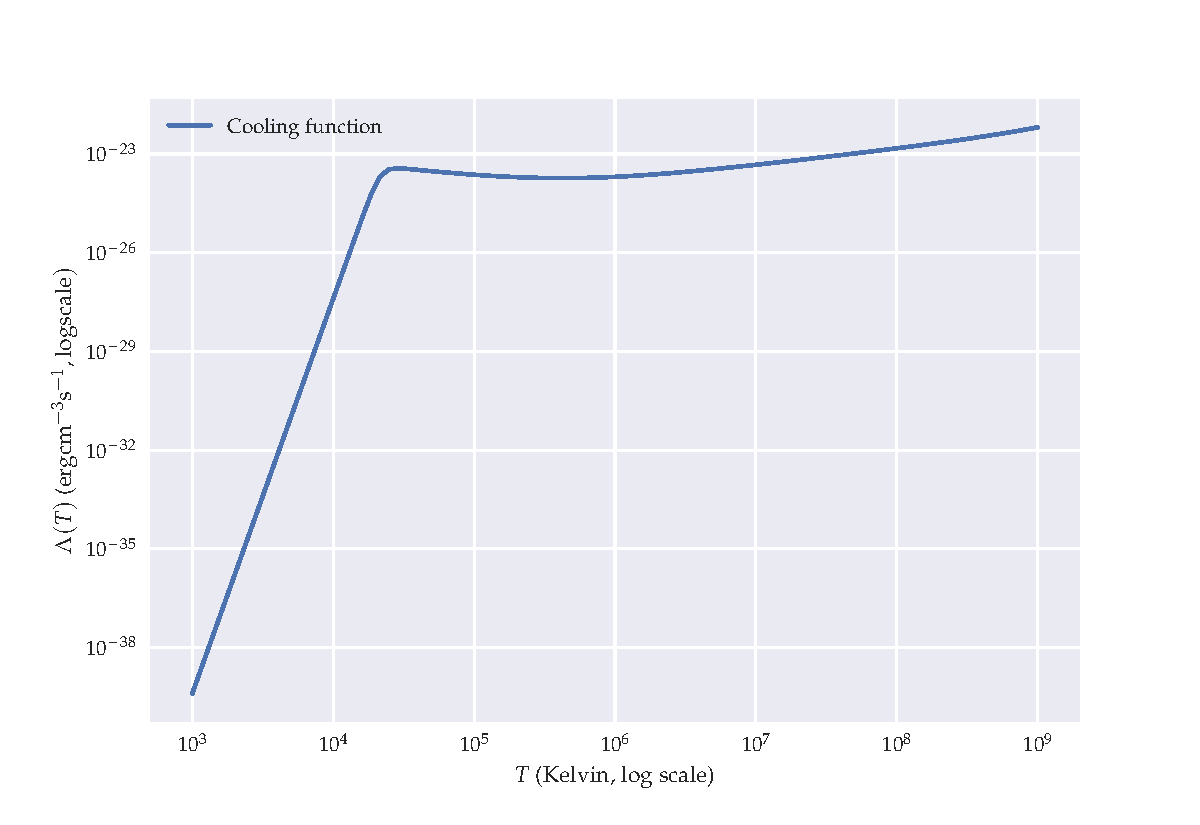
\includegraphics[width=\textwidth]{figures/cooling_function.pdf}
    \caption{Cooling function graph.}
    \label{fig:cooling-function}
\end{figure}
\begin{equation} \label{eq:cooling-function-NTZ91}
    \begin{split}
    \Lambda (T) &= \left(
    \qty(
    \num{1.42e-27}T^{1/2} \qty(
    1 + \num{4.4e-10}T
    ) + \num{6.0e-22}T^{-1/2}
    )^{-1} \right. \\
    & \quad \left. + \num{e25} \qty(\frac{T}{\SI{1.5849e4}{K}})^{-12}
    \right)^{-1} \si{\erg\cubic\centi\metre\per\second} \,.
    \end{split}
\end{equation}

%The version of this equation in \textcite[equation 10]{StellingwerfBuff:1982} is similar: the first constant is \(\SI{2.4e-27}{} \) instead of \(\SI{1.42e-27}{} \), and the factor \(\qty(1 + \SI{4.4e-10}{}T)\) is just \(1\).

\paragraph{How the conservation equations change using the moment equations}

The way we use the grey moment equations \eqref{eq:NTZ91-moment-equations-logarithmic} to study the accretion problem is by using them to simplify the conservation equations \(\nabla_\mu T^{\mu\nu}\).

The full energy momentum tensor of the problem is given, in the fiducial reference frame, by combining an ideal-fluid stress-energy tensor (with pressure \(P\) and rest energy density \(\rho\)) with the one given in \eqref{eq:radiation-stress-energy-tensor-fiducial}:

\begin{equation}
    T^{\mu\nu} =
    T^{\mu\nu}_{\text{radiation}} +
    T^{\mu\nu}_{\text{matter}} =
    \left[\begin{matrix}\rho + w_{0} & w_{1} & 0 & 0\\w_{1} & P + \frac{w_{0}}{3} + w_{2} & 0 & 0\\0 & 0 & P + \frac{w_{0}}{3} - \frac{w_{2}}{2} & 0\\0 & 0 & 0 & P + \frac{w_{0}}{3} - \frac{w_{2}}{2}\end{matrix}\right] _{\text{fid}}\,.
\end{equation}

The \(t,r\) by \(t, r\) components of the stress-energy tensor with contravariant indices in spherical coordinates are:

\begin{equation} \label{eq:spherical-coordinates-full-stress-energy-tensor}
      \left[
      \begin{matrix}
      \frac{\gamma^{4} \left(\rho - v w_{1} + \frac{v \left(v \left(3 P + w_{0} + 3 w_{2}\right) - 3 w_{1}\right)}{3} + w_{0}\right)}{y^{2}} &
      \gamma^{2} \left(- \frac{v \left(3 P + w_{0} + 3 w_{2}\right)}{3} + v \left(- \rho + v w_{1} - w_{0}\right) + w_{1}\right)\\
      \gamma^{2} \left(- v \left(\rho + w_{0}\right) + \frac{v \left(- 3 P + 3 v w_{1} - w_{0} - 3 w_{2}\right)}{3} + w_{1}\right) &
      y^{2} \left(P - v w_{1} + v \left(v \left(\rho + w_{0}\right) - w_{1}\right) + \frac{w_{0}}{3} + w_{2}\right)
    \end{matrix}
      \right] \,.
\end{equation}

\paragraph{The total luminosity \(\dot{E}\)}

We can project the conservation of the stress energy tensor along the unit vector in the temporal direction in the spherical reference frame, \((e_t)_\nu\): we get  \((e_t)_\nu \nabla_\mu T^{\nu\mu} = \nabla_\mu T_0^\mu = 0\).

Then, applying \eqref{eq:covariant-divergence} and our symmetry assumptions:

\begin{equation}
  0=\nabla_\mu T_t^{\mu}
  = \frac{1}{r^2 \sin \theta} \pdv{}{r} \qty(r^2 \sin\theta T_t^{r})
  = \frac{1}{r^2} \pdv{}{r} \qty(r^2 T_t^{r})
  \implies
  r^2 T_t^{r} = \const \,.
\end{equation}

In \cite[before eq. 18c]{ThorneFLammmangZytkow:1981feb} this appears with an additional immaterial factor of \(4 \pi\).

The quantity which is conserved is \(r^2 g_{tt}T^{tr}\), where \(T^{tr}\) is the $(0,1)$ matrix element which appears in \eqref{eq:spherical-coordinates-full-stress-energy-tensor}. We can simplify it by expressing it in terms of the luminosity \(L\) which is \(L = 4 \pi r^2 w_1\): we get

\begin{equation}
  4 \pi r^2 g_{tt} \qty(\gamma^2 (1+ v^2) \frac{L}{4 \pi r^2} - v \gamma^2 \qty(p + \rho + w_2 + \frac{4}{3} w_0)) = \const\,.
\end{equation}

We can also substitute in the expression for \(v = \dot{M} / \qty(4 \pi r^2 \rho_0 y) \), and recognize the expression for the specific enthalpy \(h\) and for \(y^2 =- g_{tt} \gamma^2\):

\begin{equation}
    -y^2 (1+v^2) L + y \dot{M} \qty(h + \frac{4w_0/3 + w_2}{\rho_0}) \defeq -\dot{E}
    = \const\,.
\end{equation}

This is the total luminosity of the accretion process.

\paragraph{The full equations of motion}

The conservation of the stress-energy tensor can be projected onto \(\hat{t}\) and \(\hat{r}\) and cast into \cite[eq. A7]{NobiliTurollaZampieri:1991dec}:

\begin{subequations} \label{eq:fiducial-projected-conservation}
\begin{align}
    (P+\rho) \dv{y}{r}
    +y \dv{P}{r}
    \underbrace{
    +\frac{4}{3} w_{0} \dv{y}{r}
    +\frac{1}{3} y \dv{w_0}{r}
    +\frac{1}{y v r^{2}} \dv{}{r}\left(y^{2} v^{2} r^{2} w_{1}\right)
    +\frac{1}{r^{3}} \dv{}{r}\left(r^{3} y w_{2}\right)}_{s_1} &=0 \\
    \dv{\rho}{r}
    -\frac{P+\rho}{\rho_{0}}
    \dv{\rho_{0}}{r}
    \underbrace{
    +\dv{w_0}{r}
    +\frac{4}{3} \frac{w_{0}}{y v r^{2}} \dv{}{r}\left(y v r^{2}\right)
    +\frac{1}{y^{2} v r^{2}} \dv{}{r}\left(y^{2} r^{2} w_{1}\right)
    +w_{2} \frac{r}{y v} \dv{}{r}\left(\frac{y v}{r}\right)}_{s_0/(yv)} &=0
\end{align}
\end{subequations}
%
where the identifications come from a reframing of the moment equations \eqref{eq:NTZ91-moment-equations-logarithmic} (see \cite[eq. A8]{NobiliTurollaZampieri:1991dec}).

By adding the continuity equation \eqref{eq:differential-continuity} to the equations \eqref{eq:fiducial-projected-conservation} --- which are reworked slightly to get the expressions of logarithmic derivatives --- we get the full system of the simplified conservation equations we will work with. Here, as in \cite[]{NobiliTurollaZampieri:1991dec} and as in section \ref{par:adiabatic-equations-of-motion}, primes denote differentiation with respect to \(\log r\).
%
\begin{subequations}
\begin{align}
  (P + \rho) \frac{y'}{y} + P^\prime + \frac{r s_1}{y}  &= 0  \\
  \rho^\prime - (P + \rho) \frac{\rho_0^\prime}{\rho_0} + \frac{r s_0}{vy}   &=0  \\
  \frac{(vy)^\prime}{vy} + \frac{\rho_0 ^\prime}{\rho_0} + 2 &=0
\end{align}
\end{subequations}

We can expresse these in terms of the variables \((yv)(r)\), \(\rho_0(r)\) and \(T(r)\).
To this end, we apply the same manipulations used in section \ref{par:adiabatic-equations-of-motion} and thus get \cite[eqs. 15]{NobiliTurollaZampieri:1991dec}:
%
\begin{subequations} \label{eq:simplified-full-equations-of-motion}
\begin{align}
  (v^2 - v_s^2) \frac{(yv) ^{\prime}}{yv} - 2 v_s^2 + \frac{M}{y^2 r}
  + \frac{r}{yv (p + \rho)} \qty((\Gamma-1)s_0 + v s_1) &= 0  \\
  \frac{T ^{\prime}}{T} - (\Gamma - 1)\frac{\rho_0 ^{\prime}}{\rho_0} - \frac{r s_0}{Bvy (p+\rho)}  &= 0  \\
  \frac{(yv) ^{\prime}}{yv} + \frac{\rho_0 ^{\prime}}{\rho_0} + 2 &=0
\end{align}
\end{subequations}
%
where \(\Gamma\), \(B\), and \(v_s^2\) are those defined in section \ref{par:adiabatic-equations-of-motion}.

\begin{greenbox}
  The sign of the source term in the energy equation is a minus: why? it seems like it should be a plus. To get the first equation, however, we need the minus.
\end{greenbox}

Their expressions will in general be unknown: they are however defined in terms of derivatives of \(\rho\) and \(p\), so if we can write an equation for those variables in terms of \(T\) and \(\rho_0\) we can compute all the desired thermodynamic variables. The desired equations of state, which need to account both for slow-moving and fully relativitic regimes, are \cite[eqs. 16]{NobiliTurollaZampieri:1991dec}:
%
\begin{subequations}
\begin{align}
  p &= \qty(1 + \frac{F}{1+F}) \frac{\rho_0 k_B T}{m_p}  \\
  \rho &= \rho_0 +  \qty( \frac{3}{2} \frac{F}{(1+F)} + \qty(\frac{\eta-1}{\theta} - 1)) \frac{\rho_0 k_B T}{m_p} + \qty(1 - \frac{F}{1+F} ) \frac{\rho_0 E_H}{m_p}
\end{align}
\end{subequations}
%
where \(F = 2 (T/\SI{1}{K}) \exp(\SI{-1.58e5}{K}/T)\) and the quantity \(F/(1+F)\) is the approximate degree of collisional ionization, \(\theta = k_B T / m_e\) while \(\eta\) is defined with the use of the Bessel functions of order \(n\), \(K_n\):  \(\eta = K_3 (\theta^{-1}) / K_2 (\theta^{-1})\); \(m_p\) and \(m_e\) are the masses of the proton and of the electron, \(k_B\) is the Boltzmann gas constant, while \(E_H\) is the Hartree energy (?).

\paragraph{Closures and singularities}

The full system of differential equations which has to be solved is composed of the two grey moment equations \eqref{eq:NTZ91-moment-equations-logarithmic}, the three equations of motion \eqref{eq:simplified-full-equations-of-motion}, plus the equation for the radiation temperature \eqref{eq:T-gamma-differential-equation}, to be solved in the six unknowns \(w_0, w_1, \rho_0, yv, T, T_\gamma\).

The shear moment \(w_2\) also appears in the grey moment equations \eqref{eq:NTZ91-moment-equations-logarithmic}, but it cannot be determined simultaneously. A \emph{closure relation} is a reasonable approximation for the behaviour of \(w_2\): what is assumed is
%
\begin{equation}
  w_2 = f(\tau) w_0 = \frac{2}{3} \frac{1}{1+ \tau^n} w_0
\end{equation}
%
where \(\tau\) is the electron scattering optical depth, which is defined \cite[eqs. 1.25, 1.26]{RybickiLightman:2004} as the function along photon paths such that the incoming intensity diminishes as \(I = I_0 e^{-\tau}\); \(f(\tau)\) is called the variable Eddington factor, while \(n \in \mathbb N\) can be chosen to reproduce different behaviours.
The error introduced by this approximation is typically of the order of \(\SI{15}{\percent}\) \cite[]{TurollaNobili:1988}.

The flow is called optically thick when, along a typical photon path (which in our case will be radial) \(\tau \gg 1\), and optically thin when \(\tau \sim 0\).
In these two cases \(f(\tau)\) approaches 0 and \(\frac[i]{2}{3}\) respectively.

If we substitute the closure relation into the grey moment equations \eqref{eq:NTZ91-moment-equations-logarithmic} and solve for \(w_l\), where \(l=0,1\), we get an equation of the form \cite[eq. 18]{NobiliTurollaZampieri:1991dec}:

\begin{equation}
  \qty(v^2 - v f(\tau) - \frac{1}{3}) w_l^{\prime} = \text{a function of }\, r, w_0, w_1, v, v', l \,.
\end{equation}

This adds a singularity to the system beyond the one at \(v=v_s\) discussed in section \ref{par:adiabatic-equations-of-motion}. This singularity is located at the zeroes of the Legendre polynomial \(P_2 (v)\) (see \eqref{eq:legendre-polynomials}, the order of the polynomial is \(2 = 1+ l_{\text{max}}\) where \(l_{\text{max}}=1\) is the maximum order of moments considered) in the optically thick limit, and at \(v \rightarrow 1\) in the optically thin limit.

\paragraph{Boundary conditions}

To solve the differential equations boundary conditions must be provided, both at the horizon and at infinity. Here are the conditions used by \textcite[]{NobiliTurollaZampieri:1991dec}.

At radial infinity we suppose there is radiative equilibrium (\(s_0 = 0\)) and the density gradient vanishes (\(\frac[i]{\rho_0 ^{\prime}}{\rho_0} = 0 \)), so by the energy equation:
%
\begin{equation}
  \frac{T ^{\prime}}{T} (r \rightarrow \infty) = 0\,.
\end{equation}

Also, we assume the energy density and energy flux decay as \(r^{-2}\): \(w_0,w_1 \propto r^{-2}\), or
%
\begin{equation}
  \frac{w_0 ^{\prime}}{w_0} (r \rightarrow \infty) = \frac{w_1 ^{\prime}}{w_1} (r \rightarrow \infty) = -2\,.
\end{equation}

At radial infinity the effects of Comptonization are negligible: this is expressed as
%
\begin{equation}
  T(r \rightarrow \infty) = T_\gamma (r \rightarrow \infty)\,.
\end{equation}

All the previous conditions are fixed, and we have a residual degree of freedom: we can look at different accretion rates \(\dot{M}\), which amounts to fixing the density
\(\rho_0\) at a certain radius,\footnote{This follows from the continuity equation  \eqref{eq:mass-conservation-integral}: since the two variables are bound by an equation, fixing one also fixes the other.} we choose the horizon:
%
\begin{equation}
  \rho_0(r = 2M) = \rho_{0, \text{hor}}\,.
\end{equation}

Conditions must be assigned at the singularities of the Jacobian of the system: we shall not explore those here, but they can be found at the end of section 3 of \cite[]{NobiliTurollaZampieri:1991dec}.

Lastly, we must fix the constant mass of the black hole \(M\): the results are generally not scale-independent, so this is actually an important choice. \textcite[]{NobiliTurollaZampieri:1991dec} chose a value of
%
\begin{equation}
    M = 3 M_{\odot}
\end{equation}
%
where \(M_\odot \approx \SI{2e30}{kg}\) is the mass of the Sun.

\paragraph{Complement: Eddington luminosity}

It is the characteristic luminosity at which the radiation pressure from the photons moving outward equals the gravitational specific force on the infalling matter.

The gravitational force, in the newtonian  limit, is

\begin{equation}
  F_{\text{grav}} = \frac{GMm}{r^2 }\,.
\end{equation}

The radiation pressure can be given in terms of the luminosity \(L\) (reinserting the units of \(c\) for this) as

\begin{equation}
  P_{\text{rad}} = \frac{L}{c 4 \pi r^2}\,,
\end{equation}
then, the radiative force is given by \(F_{\text{rad}} =  P_{\text{rad}} \kappa m\), where \(m\) is the mass of the test object and \(\kappa\) is the opacity: the per-unit-mass cross-section. We usually assume \(\kappa = \sigma_T/m_p\), that is, that the interaction between radiation and matter is all due to Thompson scattering and the matter is only composed of hydrogen atoms.

Equating the forces, we get our result:

\begin{equation}
 \frac{L_{\text{Edd}}}{M} = \frac{4 \pi c G}{\kappa}\,.
\end{equation}

In the \(\kappa = \sigma_T / m_p \approx \SI{0.04}{\metre^2 / kg}\) case, we get \(L_{\text{Edd}} / M\) to be around \SI{6.32}{\watt\per\kilo\gram} (constants' values from \cite[]{NISTReccomendedConstants:2018}).
If we express this in units of \(L_{\odot} / M_{\odot} \approx \SI{1.93E-04}{\watt\per\kilo\gram}\) \cite[]{SunFactSheet:2018} we get \(L_{\text{Edd}} / M \approx  \num{3.27E+04} L_{\odot} / M_{\odot}\):
the amount of radiation emitted by the Sun is much less than the Eddington limit.

It is, of course, important to note that this is a limit found with many approximations: nonrelativistic gravity, spherical symmetry, only Thompson scattering,
only hydrogen.

\paragraph{Solutions}

The solutions of the differential equation system, obtained numerically, include the profiles of many variables, of which a particularly interesting one is the variation of the luminosity \(L = 4 \pi r^2 w_1\) with respect to the accretion rate \(\dot{M}\).
To plot these adimensional units are used: the luminosity is rescaled by the Eddington luminosity, defining \(l = L / L_{\text{Edd}}\); the accretion rate can also be rescaled by the luminosity if we are working in natural units (otherwise we would need to use \(\dot{M}_{\text{Edd}} c^2 = L_{\text{Edd}}\)), defining \(\dot{m} = \dot{M} / L_{\text{Edd}}\). The results are shown in figure \ref{fig:logl-logm}.

\begin{figure}[ht]
    \centering
    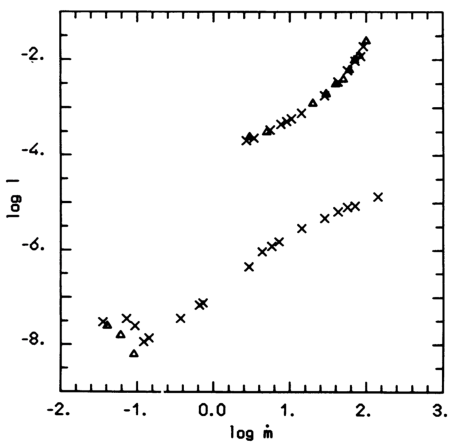
\includegraphics[width=0.7\textwidth]{figures/logl-logm.pdf}
    \caption{Log-log plot of the luminosity against the accretion rate. The crosses are the results of the simulations by \textcite[]{NobiliTurollaZampieri:1991dec}, the triangles are the results of the simulations by Park (1990a). Image credit: \cite[fig. 1]{NobiliTurollaZampieri:1991dec}.}
    \label{fig:logl-logm}
\end{figure}

The ratio between \(l\) and \(\dot{m}\) is called the \emph{efficiency} \(e\), and it represents the fraction of the mass of the infalling gas which gets converted to energy in the accretion process.

The numerical solutions for spherical accretion show two branches: the high-luminosity one has \(e \sim \num{5e-5} \divisionsymbol \num{9e-5}\), while the low-luminosity one has \(e \sim \num{9e-8} \divisionsymbol \num{9e-7}\).

In non-radial motion around a Schwarzschild black hole the efficiency can be as high as \(e \sim \num{5.7e-2}\) \cite[eq. 2.8.5]{Nobili:2000}.

This shows that, in general, spherical accretion has a very low luminosity.

\end{document}
